\chapter{Architecture}
This chapter describes the software architecture of the game prototype. It contains architectural drivers, patterns, views and tactics.

\section{Architectural Drivers}
This section will describe the motivation behind the architecture, the expected life time of the game prototype, and limitations for the implementation.

\subsection{Motivation}
The game prototype would be played by children, so the game controls and gameplay had to be easy to understand. The author also wants the game to be easy to develop for, so the game had to be easy to modify and add new features. This set the focus for the quality attributes usability and modifiability. With high usability it should be easy for the children to enjoy the game without being frustrated by the controls or gameplay elements. Focusing on modifiability it should be easy for the developer to add new features, like enemies, items, and levels.

\subsection{Expected Life Time}
The game prototype will be developed for a play testing session during the course of this project, after which the development will end. The game will not be ready for release and will be a purely gameplay prototype without a story, menus or other common non-gameplay elements. It should be possible for the author or someone else that wants to continue the project to continue working on it after the termination of this master thesis. Information on possibilities for future work is detailed in Chapter \ref{chp:further_work}.

\subsection{Limitations}
The game will be developed using Unreal Engine 4, so the project will be limited to use of the underlying architecture of that engine. Included in the engine is a plugin called Paper2D that will be used, which helps with the creation of 2D games. The author has no previous experience with Unreal Engine, which presented challenges and opportunities to develop new skills. 


\section{Unreal Architecture}
The Unreal Engine uses a modular architecture where the engine is comprised of different modules for elements like networking, shaders, and physics. In a projects settings, the developer can define the different modules that are needed. When creating a game, the developer will mostly be working with the gameplay framework of the engine. The following sections describe the gameplay framework. The information presented is taken from the Unreal Engine's online documentation \cite{epicgames2016doc}.

\subsection{Players and Entities}
All visual objects in the game world, like players, enemies, and items all share the base class Actor. An Actor is basically any object that can be placed into a level, they support basic 3D transformations, such as translation, rotation and scale. The Pawn class is the base class for all Actors that can be controlled by players or \gls{ai}, and are set up to easily accept input. Character is the class for representing a humanoid-style Pawn, which has a component for movement and collision detection.

\subsection{Control and Input}
There are two main ways of controlling a Pawn, by using a PlayerController or an AIController. Both classes share the base class Controller. The Controller is responsible for directing the Pawn which is referred to as possessing a Pawn. The PlayerController is the interface between the Pawn and the player, it handles the input from the player and issues commands to the Pawn. The AIController class responds to input from the game environment and uses \gls{ai} logic to command the Pawn.

\subsection{Display}
There is a HUD class which is the base class for displaying elements overlaid on the screen. Every PlayerController has an instance of the HUD class which draws their individual viewport. The Playercontroller also has an instance of a PlayerCameraManager class, which represents the view of the player.

\subsection{Game Rules}
The rules of the game are defined and implemented in a GameMode class. A game should implement functions or variables that set or enforce game rules in a subclass of the GameMode class. There can only be one game mode at any given time, and in the context of networking games, the GameMode will only be present on the server. GameState contains the state of the game, which can include the score, location of chess pieces in a chess game, or what tasks have been completed. There is also a class called PlayerState for keeping track of the state of a player in the game. Things like player name, experience level or score are data that would be present in the PlayerState.

\subsection{Game Framework Overview}
Figure \ref{fig:game_framework} shows how the gameplay classes interact with each other. The game is made up of a GameMode which sets and enforces the game rules and a GameState which describes the state of the game. Players are represented by PlayerControllers which can possess Pawns in order to control them. Pawns can also be controlled via an AIController that controls the Pawn using \gls{ai}. The PlayerController provides the player with input controls for controlling the pawn, a HUD for displaying an overlay on the screen, and a PlayerCameraManager for handling the players view in the game world.

\hfigure{game_framework}{The relationship between the game framework classes \cite{epicgames2016framework}}{1}


\section{Game Architecture and Views}
The architecture for the game is based on the Unreal Engines architecture and uses C++ classes and Blueprints. All classes and Blueprints inherit from a class in the Unreal Engine framework. Figure \ref{fig:class_diagram_full} shows the inheritance between classes and illustrates how the games architecture is linked with the architecture of Unreal Engine. The classes are organized into directories which form different groups of classes. The following sections will explain these groups in greater detail. The folder structure of the C++ game source is illustrated in Figure \ref{fig:package_diagram_source}.

\hfigure{package_diagram_source}{The folder structure of the source files}{0.7}

\begin{sidewaysfigure}[!ht]
	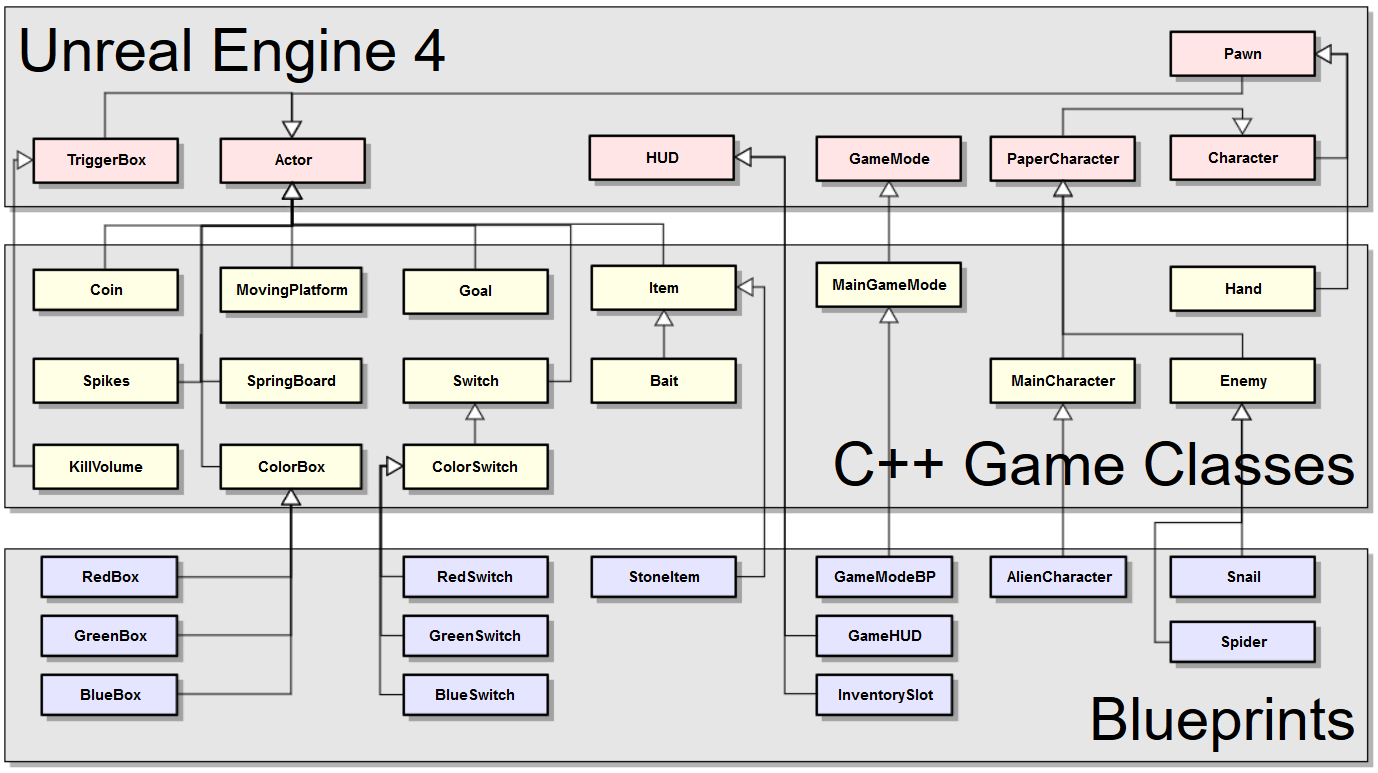
\includegraphics[width=\textwidth]{images/class_diagram_full}
	\caption{Class diagram for all the classes of the game prototype}
	\label{fig:class_diagram_full}
\end{sidewaysfigure}

\subsection{World Objects}
The world objects are static objects that exist in the game world that the character or the hand can interact with. The classes that are grouped as world objects are Coin, Goal, MovingPlatform, Spikes, SpringBoard, KillVolume, Switch, ColorSwitch and ColorBox. Most of these represent gameplay elements that are explained in Section \ref{sec:gameplay_elements}. KillVolume is a trigger to kill the character when it moves out of bounds of the game world. Goal is the goal that the character has to reach in order to complete the level. ColorSwitch inherits from Switch in order to reuse functionality. The difference between the two types of switches is that the regular Switch controls one or more MovingPlatforms and the colour switches control the existence of coloured blocks.

\subsection{Items}
Items represent the items that the character can pick up and add to the inventory. There are currently only two classes of items: the Item class and the Bait class. The Item class is made in such a way that it is easy to subclass it and alter the functionality of a new type of item. The Bait class does this and only alters two functions from the Item class.

\subsection{Game}
The game category only consist of the MainGameMode class. Becase the game prototype does not have very complex rules or game states, and there is no need for networking, the functionality in the MainGameMode includes functionality that normally belongs in the GameState. For the same reasons, there are also no PlayerStates. The MainGameMode handles the display of the HUD, keeps track of the score and inventory, and what item is currently grabbed by the hand.

\subsection{Characters}
The characters are the classes that move around in the game world and consist of the MainCharacter, Hand, and Enemy classes. These classes are sub-classes of PaperCharacter which is a specialization of the Character, found in the Paper2D plugin. Normally non-human controlled pawns are not Characters, but the enemies share similar movement and collision detection of the player, so they were made into characters.

\subsection{Blueprints}
The blueprints were used in such a way that they only changed a few attributes of their super-classes. All the blueprints, except for the HUD blueprints, were based on a C++ class where the majority of the functionality existed. Most of the additions of the Blueprints were minor, like using a different sprite, or changing the movement speed of an enemy. Blueprints were convenient for this because of the ease of changing attributes while testing the game. Using Blueprints helps with the modifiability, by making it easy to change attributes and appearance of the different game elements.

%\section{Tactics}
%modifiability
%usability

\section{Summary}
The motivation for the architecture is to focus on high usability and modifiability. Usability is achieved in part by using the Unreal Engine to handle controller input, physics, collision and rendering which makes for a smooth gameplay experience. The other part of usability is to make sure that the gameplay elements implemented are fun, yet challenging. Modifiability is ensured by making the gameplay elements easily extendible through C++ classes of Blueprints. The Unreal Engine's gameplay framework also promotes modifiability by using a modular system that increases cohesion.
